% !TeX spellcheck = en_US
\documentclass[11pt,a4paper]{article}
\usepackage[utf8]{inputenc}
\usepackage{amsmath}
\usepackage{amsfonts}
\usepackage{amssymb}
\usepackage{graphicx}
\usepackage{mathtools}
\usepackage[hidelinks]{hyperref}  % most people dont know of this :3

\usepackage{subfig}
\usepackage[margin=0.7in]{geometry}

% \usepackage[backend=bibtex,style=verbose-ibid]{biblatex}
% \addbibresource{citations.bib}

\usepackage{listings}
\usepackage{color}
\definecolor{dkgreen}{rgb}{0,0.6,0}
\definecolor{gray}{rgb}{0.5,0.5,0.5}
\definecolor{mauve}{rgb}{0.58,0,0.82}

\lstset{frame=tb,
  language=Python,
  aboveskip=3mm,
  belowskip=3mm,
  showstringspaces=false,
  columns=flexible,
  basicstyle={\small\ttfamily},
  numbers=none,
  numberstyle=\tiny\color{gray},
  keywordstyle=\color{blue},
  commentstyle=\color{dkgreen},
  stringstyle=\color{mauve},
  breaklines=true,
  breakatwhitespace=true,
  tabsize=3
}


\newcommand{\inv}{^{\raisebox{.2em}{$\scriptscriptstyle-1$}}}
\newcommand{\qed}{\hfill $\blacksquare$}

\newcommand{\integers}{\mathbb{Z}}
\newcommand{\rationals}{\mathbb{Q}}
\newcommand{\reals}{\mathbb{R}}
\newcommand{\complexes}{\mathbb{C}}
\newcommand{\field}{\mathbb{F}}

\author{Jacob Bruner}
\title{Bivariate Statistics Exploration}
\date{\today}

\begin{document}
\maketitle
% \tableofcontents

% \pagebreak

\iffalse
############
heres an example of a code block
\begin{lstlisting}
        def intervalValues(z, n):
            return output # return the sequence of values
\end{lstlisting}

heres an example of an image
\begin{figure}[h]
\begin{center}
\includegraphics[scale=.37]{onefifteen} 
\caption{Sequences Generated by n = 1-15 on Argand Diagram}
\end{center}
\end{figure}
############
\fi

\section{Introduction}

In the real-world, statistics are often employed as objective measures of data. Because of this, we often draw important decisions on their basis alone. For instance, pharmacists employ statistics when researching new treatments for disease, or economists might draw on statistics to understand trends in consumer spending. Luckily for us, statistics often \textit{are} helpful and insightful in disseminating patterns in data. But, again, it is all too easy to forget their short-comings.

In 1973, British mathematician Francis Anscombe formulated four datasets, each with 11 points, in order to demonstrate the pitfalls of many common statistical measures. (See Table~\ref{fig:datas} in the Appendix, page \pageref{Appendix}.) In this paper, I will explore the ways in which these statistical measures can be misleading in interpreting the significance of, trends in, or validity of data using Anscombe's 'quartet' of points to highlight their oversimplification.

\section{The Statistical Mean}
\subsection{Computation}
The mean is a commonly used measure of center for a given dataset. To calculate the mean, we can use the following formula: for a given indexed set of values, the mean is written:
\[
\bar{x} = \frac{1}{N} \sum_{i = 1}^{N} x_i
\]
Where N is the length of the data set. In other words, the mean is the sum of each value divided by the number of values for a given parameter. \\


Calculating these values for each dataset in Anscombe's Quartet we obtain:

\begin{figure}[ht]
\centering
\begin{tabular}{|l|cc|cc|cc|cc|}
\hline
\textbf{Data set}         & \multicolumn{2}{c|}{\textbf{I}}              & \multicolumn{2}{c|}{\textbf{II}}             & \multicolumn{2}{c|}{\textbf{III}}            & \multicolumn{2}{c|}{\textbf{IV}}             \\ \hline
\textbf{Parameter} & \multicolumn{1}{c|}{\textit{x}} & \textit{y} & \multicolumn{1}{c|}{\textit{x}} & \textit{y} & \multicolumn{1}{c|}{\textit{x}} & \textit{y} & \multicolumn{1}{c|}{\textit{x}} & \textit{y} \\ \hline
\textbf{Mean}     & \multicolumn{1}{c|}{9.0}        & 7.5        & \multicolumn{1}{c|}{9.0}        & 7.5        & \multicolumn{1}{c|}{9.0}        & 7.5        & \multicolumn{1}{c|}{9.0}        & 7.5        \\ \hline
\end{tabular}
\caption{Computed Means of $x$ and $y$ in Datasets I through IV}
\end{figure}

\subsection{Interpretation}

After computing, it's clear that the means for each $x, y$ of the respective datasets are equal. Without any other prior knowledge, one might infer that these datasets have a similar center, notwithstanding variation or spread. This is because the mean doesn't provide information about the variation or spread of the data. Despite this, however, one might assume it to be a reasonable assumption that these datasets and parameters might be highly similar, especially because they match in both variables. If these corresponded to real world data, it might be inferred that these means would be the approximate \textit{expected} result if another trial were to be performed. However, this is contested upon further inspection.

\section{Exploring Other Statistical Measures}
\subsection{Computation}

In addition to computing the mean, there are a number of other tools that provide insight into the properties of a dataset. For instance, the \textbf{\textit{variance}} ($\sigma^2$) and \textbf{\textit{standard deviation}} ($\sigma$) convey a measure of the 'spread' or variation in a dataset. Similarly, \textbf{\textit{'Peterson's Correlation Coefficient'}} ($r$) often denoted with its square, $r^2$, is measure of the \textit{linear} coorelation of two parameters. (Unsquared) values of $r$ range from -1 to 1, with numbers farther from zero denoting stronger coorelation. A closely related notion is the \textbf{\textit{covariance}}, which measures the linear coorelation, but with a magnitude not necessarily between $(-1, 1)$. These measures are related like so: $r = \frac{cov(x, y)}{\sigma_x \sigma_y}$ where $\sigma$ denotes the standard deviation. The computed values of these for Anscombe's Quartet can be found below:

\begin{figure}[ht]
\centering
\begin{tabular}{l|c|c|c|c|c|c|c|c|}
\cline{2-9}
                                     & \textbf{$\bar{x}$} & \textbf{$\bar{y}$} & \textbf{$\sigma_x^2$} & \textbf{$\sigma_y^2$} & \textbf{$\sigma_x$} & \textbf{$\sigma_y$} & \textbf{$r^2$} & \textbf{$cov(x, y)$} \\ \hline
\multicolumn{1}{|l|}{\textbf{set 1}} & 9.0                & 7.5              & 11.0                & 4.13                & 3.32                  & 2.03                  & 0.67           & 5.5                  \\ \hline
\multicolumn{1}{|l|}{\textbf{set 2}} & 9.0                & 7.5              & 11.0                & 4.13                & 3.32                  & 2.03                  & 0.67           & 5.5                  \\ \hline
\multicolumn{1}{|l|}{\textbf{set 3}} & 9.0                & 7.5              & 11.0                & 4.12                & 3.32                  & 2.03                  & 0.67           & 5.5                  \\ \hline
\multicolumn{1}{|l|}{\textbf{set 4}} & 9.0                & 7.5              & 11.0                & 4.12                & 3.32                  & 2.03                  & 0.67           & 5.5                  \\ \hline
\end{tabular}
\caption{Comparison of different Statistical Measures of Datasets I-IV}
\label{fig:table}
\end{figure}

\subsection{Plotting Data}

Using the python packages \texttt{matplotlib}, \texttt{scipy}, \texttt{numpy} and \texttt{pandas}, we can plot each dataset (as a dataframe contained in the array \texttt{dfs}). A linear regression is fit to the data using the \texttt{np.polyfit()} method with an exponent of 1, and the Pearson's coefficent is calculated using the \texttt{stats.pearsonr()} method. This is accomplished like so:

\begin{lstlisting}
for i in range(4):
  dfs[i].plot.scatter(x='x', y='y')  # create scatterplot of data
  reg = np.polyfit(dfs[i]['x'], dfs[i]['y'], 1)  # compute regression
  rval = stats.pearsonr(dfs[i]['x'], dfs[i]['y'])[0]  # compute r
  plt.plot(dfs[i]['x'], np.polyval(reg, dfs[i]['x']), 'r', label='y={:.2f}x+{:.2f}\n r^2 = {:.2f}'.format(reg[0], reg[1], rval**2)) # draw regression
  plt.xlabel('x')
  plt.ylabel('y')
  plt.legend()  # add legend
  plt.savefig('dataset{}.png'.format(i+1))
\end{lstlisting}

In so doing, we get the following interesting results (Figure~\ref{fig:plots}).

\begin{figure}[ht]
\centering
\subfloat[Dataset I]{\label{fig:I}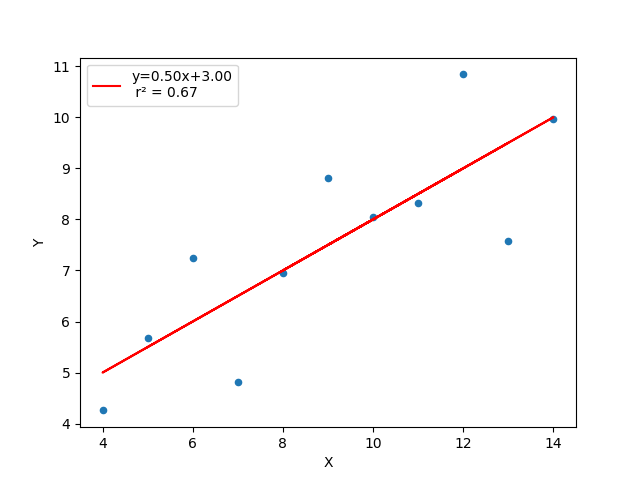
\includegraphics[width=0.45\linewidth]{dataset-1.png}}\qquad
\subfloat[Dataset II]{\label{fig:II}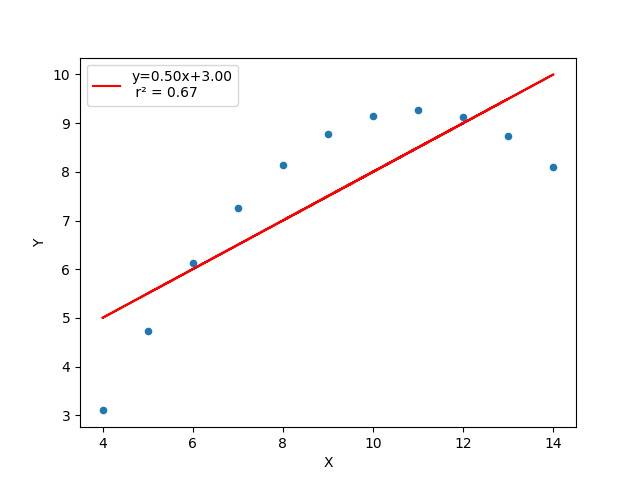
\includegraphics[width=0.45\linewidth]{dataset-2.png}}\\
\subfloat[Dataset III]{\label{fig:III}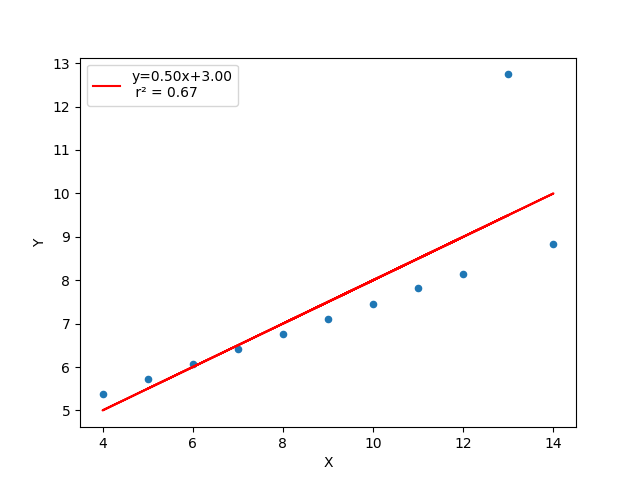
\includegraphics[width=0.45\textwidth]{dataset-3.png}}\qquad%
\subfloat[Dataset IV]{\label{fig:IV}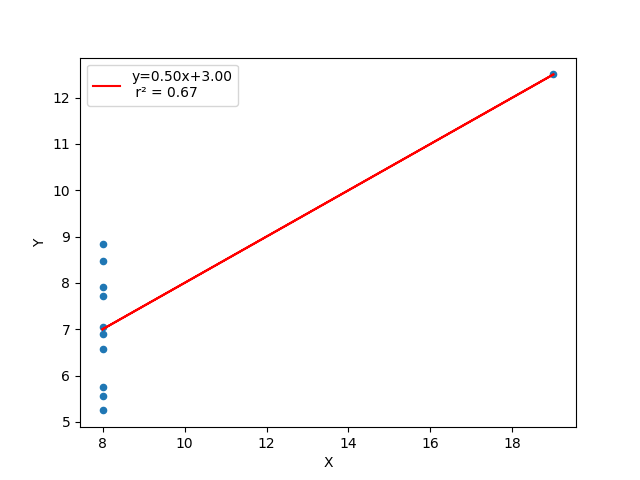
\includegraphics[width=0.45\textwidth]{dataset-4.png}}%
\caption{Plot of Datasets I-IV — X against Y with Lin. Reg.}
\label{fig:plots}
\end{figure}

\subsection{Interpretation}

Upon examination of the computed statistical measures (std, variance, cov, etc.), the naive conclusion would be that each dataset contains extremely similar data and that similar conclusions could be drawn from each. For instance, the $r^2$ value for each, $0.67$, indicates that there is a moderately-weak, positive correlation between the variables, and might imply that linear fits to each dataset would have a similar degree of inaccuracy. However, this notion is \textit{categorically refuted} on even a cursory glance at the graphs. In Figure~\ref{fig:plots}, we see that each dataset is very distinct in its scatterplot pattern. In Figure~\ref{fig:I}, its clear that the linear fit to the data indicates weak-moderate, positive correlation, with a healthy amount of deviation from the trendline. This graph's, the most straightforward of the four, statistical measures indicate helpful information about the data. For instance, the $r^2$ value of $0.67$ reinforces the weak, positive spread outlined above. Similarly, the covariance of $5.5$ and the variance $\sigma_x^2 = 11.0,\ \sigma_y^2 = 4.13$ reinforce the visual intuition of this dataset having a healthy amount of spread from the means $\bar{x}, \bar{y}$. 

	As we transition to Figure~\ref{fig:II}, we see a markedly different trend in the data. 
Visually, the scatterplot indicates an quadratic trend in $x$, indicating that the $y$ values may vary proportional to the negative square of $x$. 
Despite this, our linear trendline (from a least squares regression) provide a line of 'best fit' equal to that of Figure~\ref{fig:I}, despite the very different appearance of the data. 
Additionally, the other statistical measures of dataset II are exactly equivalent to that of dataset I, despite the visual interpretation being different. For instance, one might interpret the $r^2$ value in Figure~\ref{fig:I} as indicating the moderate (seemingly random) variation from the trendline, whereas in Figure~\ref{fig:II}, we see the datapoints follow exactly the (not random) curve of a quadratic, despite still having the same $r^2$. 
If one were to perform a polynomial regression on set II (perhaps taking the logarithm to linearize the polynomial exponent, then performing a least squares regression), the resulting trendcurve would likely be an extremely close fit to the data---a fact not illustrated by these statistical measures. 

	In Figure~\ref{fig:III}, we see a different outcome where, despite displaying a very linear trend, the computed statistics and trendline are greatly affected by a single outlier. Because of this, we see the trendline having the incorrect slope to match the (linear) trend in the rest of the data. Despite this outlier not being indicated in the computed statistical measures, viewing the graph demonstrates the highly linear relationship between x and y, which would be easily illustrated by removing the outlier or otherwise explaining it in the methodology. This fact highlights the difference between dataset III and dataset I, where, despite having the same statistical measures, Figure~\ref{fig:I} displays almost uniformly random deviation from the line of best fit compared to Figure~\ref{fig:III} which has a nicely behaved deviation given by the intersection of another trendline if the sole outlier were to be removed.
This discrepancy may be a result of the priority of a least squares regression, \textit{optimizing the squared distance to a regression line}. This method is biased towards extrema in the data, because it is optimizing the \textit{squared} deviation, abnormally increasing the influence of the outlier in III.

	In Figure~\ref{fig:IV}, dataset IV, we see how the statistical measures fail to indicate that most of the measured independent '$y$' values coorespond to a single dependent '$x$' value, namely $8$. Notwithstanding this, we can still obtain a 'regression line' of sorts, which attempts to interpret this data as being linear. Clearly, from the scatterplot, this regression is wishful thinking \textit{at best}, and complete nonsense at worst. Despite the other datasets indicating some relationship/coorelation between $x$ and $y$, the grouping of $y$s at $x=8$ indicates no such  obvious relationship. Despite this, the numerical methods of a linear regression can still be performed, wrongfully indicating much similarity between dataset IV and datasets I-III.

\section{Additional Areas to Explore}
\subsection{Residual Plots}

Other tools are available in statistics to help better draw conclusions about unintuitive datasets like Ascombe's Quartet. One such method is the use of residuals when plotting a regression. By slightly modifing the code above, one can run:

\begin{lstlisting}
for i in range(4):
  #  + code from before
  residuals = dfs[i]['y'] - np.polyval(reg, dfs[i]['x']) # compute residuals
  plt.scatter(dfs[i]['x'], residuals, c=residuals, cmap='seismic', vmin=-3, vmax=3,s=15)  # add residuals
  plt.axhline(y=0, color='r', linestyle='--', linewidth=1)  # add red line
  plt.colorbar()  # add colorbar
\end{lstlisting}
Obtaining:
\begin{figure}[ht]
\centering
\subfloat[Dataset I]{\label{fig:rI}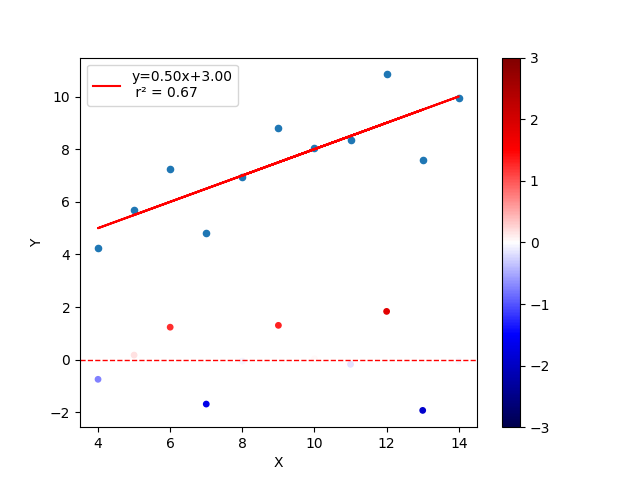
\includegraphics[width=0.45\linewidth]{dataset-res-1.png}}\qquad
\subfloat[Dataset II]{\label{fig:rII}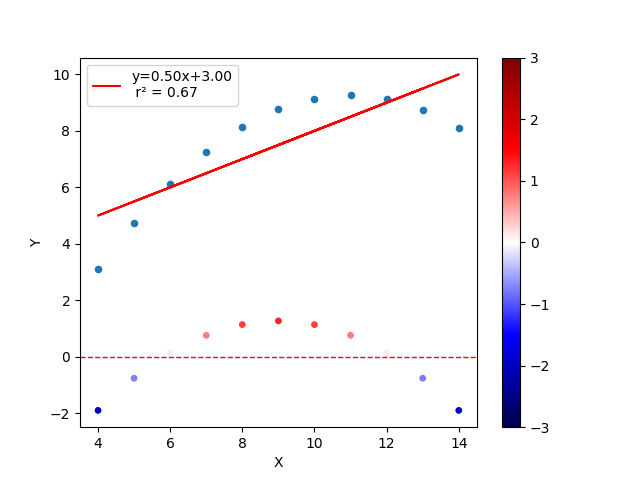
\includegraphics[width=0.45\linewidth]{dataset-res-2.png}}\\
\subfloat[Dataset III]{\label{fig:rIII}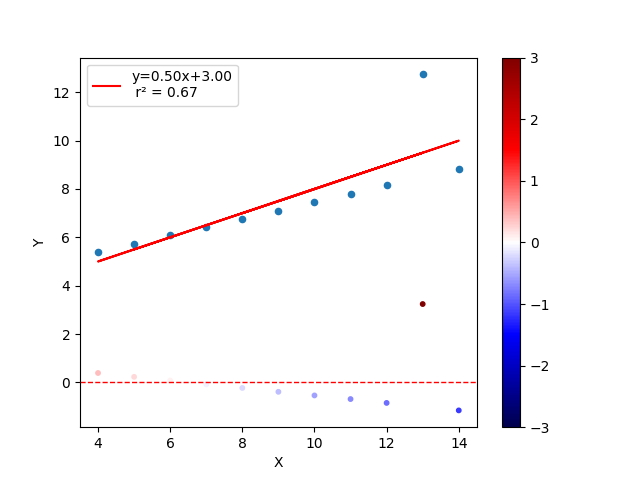
\includegraphics[width=0.45\textwidth]{dataset-res-3.png}}\qquad%
\subfloat[Dataset IV]{\label{fig:rIV}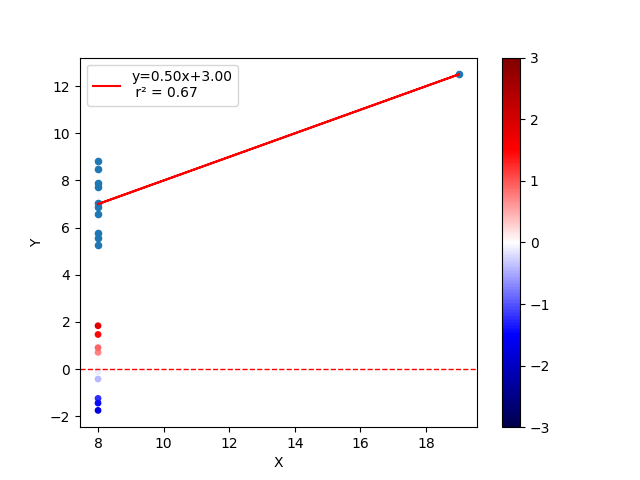
\includegraphics[width=0.45\textwidth]{dataset-res-4.png}}%
\caption{Residuals Plot of Datasets I-IV — X against Y with Lin. Reg.}
\label{fig:rplots}
\end{figure}
\linebreak
After viewing the residual plots, it's clear that scrutinizing the pattern of residuals could be an insightful method at determining the reliability of a regression. For instance, one could compare the  datasets II and II with that of dataset I by determining that the computed regressions aren't appropriate to datasets II and III because there are clear patterns in the residuals. In Figure~\ref{fig:rI}, there seems to be a healthy randomness in the distribution of residuals, corresponding to the natural variation in the parameters from the trendline. Whereas in Figures~\ref{fig:rII}-\ref{fig:rIII}, there is a quadratic and linear pattern respectively in the residuals. Hence, one could infer that there would be a better fit to each dataset by considering other factors (a non-linear regression and outlier influence here respectively, for instance). Similarly the residuals in Figure~\ref{fig:rIV} confirms that this regression line is a poor model for the data, since almost every datapoint occurs at $x = 8$, creating a vertical column of residuals and an absence of such everywhere else.

\subsection{Arguments for Graphing Before Interpretation}

To expand this investigation, another important question is whether one must graph data before analyzing. From the results of this exploration, one could argue that graphs provide visual insight that cannot be captured within measures like a mean, standard deviation, or $r^2$ value. We see that all four datasets evaluate to the same statistical values in Table~\ref{fig:table} despite having  markedly different graphs. For this reason, for datasets where graphing is an option, one would conclude that graphing should absolutely be employed before interpreting statistics of a dataset. However, in certain applications where graphing isn't as easy (for instance multi-variate data), it might be out of necessity that statistical measures are interpreted without visual aid. However, as evidenced by this exploration, this may lead to misinterpretation of the results.

\section{Conclusion}

Despite the interpretation of statistics as 'objective measures,' this exploration highlights how certain datasets may be misinterpreted and misunderstood with statistical analysis because of hidden factors. Before being able to visually interpret the data, relying on the computed statistics (mean, $\sigma,\ \sigma^2,$ cov, $r^2$) alone may not be sufficient to draw substantiated conclusions. The conclusion to be drawn from this exploration is that these measures \textit{necessarily} have to simplify the dataset, causing a loss of information which can conceal certain facts about the data. This is because, no matter what, these statistics reduce an entire set of data into a single number, often constrained to a certain range. Hence, statisticians must rely on crude methods (e.g., graphing a scatterplot, or visually inspecting the numbers for outliers) before drawing conclusions from a dataset, if they want to ensure the validity of their conclusions. In many instances, these reductionist measures \textit{are} reliable and indicate true facts about a dataset (for instance, in dataset I, most of the statistics convey useful facts), but it's important to confirm these within the context of the entire dataset.

\section{Appendix} \label{Appendix}

\begin{figure}[h]
\begin{center}
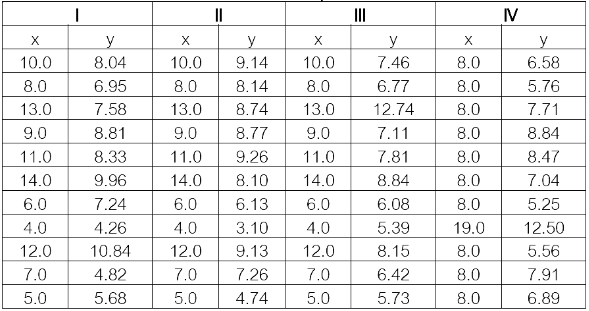
\includegraphics[scale=.65]{datatable} 
\caption{Ascombe's Quartet -- Datasets I through IV}
\label{fig:datas}
\end{center}
\end{figure}

\end{document}